\documentclass{book}    % fundamental class file is 'book'.
\usepackage{float}
\usepackage{pgf}
\usepackage{tikz}
\usetikzlibrary{shapes}
\usepackage{PGFTikzGraph}
\usepackage[hyphens]{url}
\usepackage[hidelinks]{hyperref}	% Clickable links to figures, references and urls.
\usepackage{meta}  % use the file 'meta.sty'.
\pagestyle{meta}

\begin{document}

\title{Finite Difference Time--Domain Modelling of Metamaterials: GPU Implementation of Cylindrical Cloak}
\maketitle
%===================================================

%-- Author(s) for the first affiliation ---
\author      {A. Dawood}
\affiliation {National University of Computer and Emerging Sciences (FAST)}
\address     {}% optional
\city        {Islamabad}
\postalcode  {}% optional
\country     {Pakistan}
\phone       {+92-111128128-271}    % optional
\fax         {}    % optional
\email       {attique.dawood@nu.edu.pk}  % optional
\misc        { }  % optional
\nomakeauthor
%------------------------------------

%---Output of Authors----------------------
\begin{authors}

{\bf A. Dawood}$^{1}$\\
\medskip
$^{1}$National University of Computer and Emerging Sciences (FAST), Pakistan\\
attique.dawood@nu.edu.pk
\end{authors}
%--------------------------

%---Content of Paper Abstract-----------------------
\begin{paper}

\begin{metaabstract}
Finite difference time--domain (FDTD) technique can be used to model metamaterials by treating them as dispersive material. Drude or Lorentz model can be incorporated into the standard FDTD algorithm for modelling negative permittivity and permeability. FDTD algorithm is readily parallelisable and can take advantage of GPU acceleration to achieve speed--ups of 5x--50x depending on hardware setup. Metamaterial scattering problems are implemented using dispersive FDTD technique on GPU resulting in performance gain of 10x--15x compared to conventional CPU implementation.
\end{metaabstract}
%---Content of Paper Text-----------------------
%\psection{Introduction}
Standard FDTD algorithm cannot cater for negative values of permittivity or permeability. This is because of the Courant stability criterion. As soon as the permeability or permittivity becomes less than unity the algorithm will not be stable. A metamaterial object can be modelled as a dispersive substance using either the Lorentz or Drude dispersive models. These models can yield negative values of permittivity (or permeability) for certain frequency ranges~\cite{NumericalFDTD-Sibel}. Using these dispersive models, FDTD update equations are modified and permittivity and permeabilities are replaced with terms dependent on frequency of operation.

Two problems are chosen for GPU implementation. First is the electromagnetic wave scattering by a slab with negative permittivity and permeability; also known as DNG (double negative) medium. Second problem is the simulation of cylindrical cloak. An incident Gaussian pulse on DNG slab will undergo dispersion resulting in different frequency components being separated. Refractive index and transmission coefficient are calculated numerically to ascertain the validity of implementation. The cylindrical cloak was first proposed and tested by Pendry et. al. \cite{PendryShurig-MicrowaveCloak}. The first FDTD implementation was by Zhao et. al \cite{Radial-Zhao} and implemented on Comsol, a commercial electromagnetic simulation software. Simulations are implemented on Matlab, C++ and GPU. Performance comparison reveals a 10--15 times increase in performance with GPU implementations. Performance gain is greater for larger problem sizes and greater simulation times.
\begin{figure}[H]
\mbox{
	\subfigure[DNG slab problem]
	{
	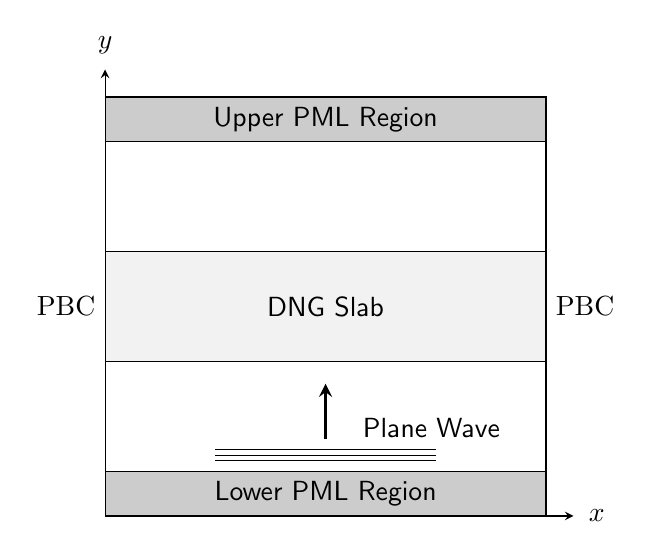
\begin{tikzpicture}[xscale=0.7,yscale=0.7]
		\newcommand{\LeftX}{0cm}
		\newcommand{\MidX}{4cm}
		\newcommand{\RightX}{8cm}
		\newcommand{\PMLw}{0.8cm}
		\newcommand{\DomainY}{6.0cm}
		\newcommand{\SlabStartY}{2.0cm+\PMLw}
		\newcommand{\SlabEndY}{4.0cm+\PMLw}
		% x-axis.
		\draw[->, >=stealth] (\LeftX,0cm) -- (\RightX+0.5cm,0cm);
		\coordinate [label=right:$x$] (x-axis) at (\RightX+0.6cm,0cm);
		% y-axis.
		\draw[->, >=stealth] (\LeftX,0cm) -- (\LeftX,2*\PMLw+\DomainY+0.5cm);
		\coordinate [label=above:$y$] (y-axis) at (\LeftX,2*\PMLw+\DomainY+0.6cm);
		% PBCs.
		\coordinate [label=right:PBC] (PBCright) at (\RightX,\PMLw+3.0cm);
		\coordinate [label=left:PBC] (PBCleft) at (\LeftX,\PMLw+3.0cm);
		% Lower PML Region.
		\draw[fill=gray!40!white] (\LeftX,0cm) rectangle (\RightX,\PMLw);
		\coordinate [label=center:\textsf{Lower PML Region}] (LowerPML) at (\MidX,0.4cm);
		% Solution Region.
		\draw (\LeftX,\PMLw) rectangle (\RightX,\PMLw+\DomainY);
		% Upper PML Region.
		\draw[fill=gray!40!white] (\LeftX,\PMLw+\DomainY) rectangle (\RightX,2*\PMLw+\DomainY);
		\coordinate [label=center:\textsf{Upper PML Region}] (UpperPML) at (\MidX,\PMLw+\DomainY+0.4cm);
		% Slab.
		\draw[fill=gray!10!white] (\LeftX,\SlabStartY) rectangle (\RightX,\SlabEndY);
		\coordinate [label=center:\textsf{DNG Slab}] (DNGSlab) at (\MidX,\PMLw+3.0cm);
		% Plane wave.
		\draw (\LeftX+2.0cm,\PMLw+0.2cm) -- (\RightX-2.0cm, \PMLw+0.2cm);
		\draw (\LeftX+2.0cm,\PMLw+0.3cm) -- (\RightX-2.0cm, \PMLw+0.3cm);
		\draw (\LeftX+2.0cm,\PMLw+0.4cm) -- (\RightX-2.0cm, \PMLw+0.4cm);
		\draw[line width=1.1pt, ->, >=stealth] (\MidX,\PMLw+0.6cm) -- (\MidX,\PMLw+1.6cm);
		\coordinate [label=right:\textsf{Plane Wave}] (PlaneWave) at (\MidX+0.5cm,\PMLw+0.8cm);
	\end{tikzpicture}
	}
	\quad
	\subfigure[Cylindrical cloak]
	{
	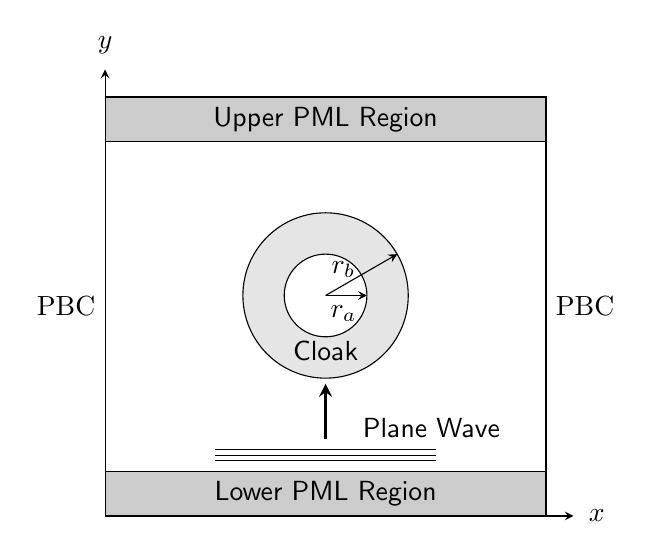
\begin{tikzpicture}[xscale=0.7,yscale=0.7]
		\newcommand{\LeftX}{0cm}
		\newcommand{\MidX}{4cm}
		\newcommand{\RightX}{8cm}
		\newcommand{\PMLw}{0.8cm}
		\newcommand{\DomainY}{6.0cm}
		\newcommand{\SlabStartY}{2.0cm+\PMLw}
		\newcommand{\SlabEndY}{4.0cm+\PMLw}
		% x-axis.
		\draw[->, >=stealth] (\LeftX,0cm) -- (\RightX+0.5cm,0cm);
		\coordinate [label=right:$x$] (x-axis) at (\RightX+0.6cm,0cm);
		% y-axis.
		\draw[->, >=stealth] (\LeftX,0cm) -- (\LeftX,2*\PMLw+\DomainY+0.5cm);
		\coordinate [label=above:$y$] (y-axis) at (\LeftX,2*\PMLw+\DomainY+0.6cm);
		% PBCs.
		\coordinate [label=right:PBC] (PBCright) at (\RightX,\PMLw+3.0cm);
		\coordinate [label=left:PBC] (PBCleft) at (\LeftX,\PMLw+3.0cm);
		% Lower PML Region.
		\draw[fill=gray!40!white] (\LeftX,0cm) rectangle (\RightX,\PMLw);
		\coordinate [label=center:\textsf{Lower PML Region}] (LowerPML) at (\MidX,0.4cm);
		% Solution Region.
		\draw (\LeftX,\PMLw) rectangle (\RightX,\PMLw+\DomainY);
		% Upper PML Region.
		\draw[fill=gray!40!white] (\LeftX,\PMLw+\DomainY) rectangle (\RightX,2*\PMLw+\DomainY);
		\coordinate [label=center:\textsf{Upper PML Region}] (UpperPML) at (\MidX,\PMLw+\DomainY+0.4cm);
		% Cloaking shell.
		\draw[fill=gray!20!white] (4cm,4cm) circle (1.5cm);
		\draw[fill=white] (4cm,4cm) circle (0.75cm);
		\coordinate [label=center:\textsf{Cloak}] (Cloak) at (\MidX,3cm);
		\draw[->, >=stealth] (\MidX,4cm) -- (\MidX+0.75cm,4cm);
		\draw[->, >=stealth] (\MidX,4cm) -- (\MidX+1.3005cm,4.75cm);
		\coordinate [label=below:$r_a$] (ra) at (\MidX+0.325cm,4cm);
		\coordinate [label=above:$r_b$] (rb) at (\MidX+0.325cm,4.15cm);
		% Plane wave.
		\draw (\LeftX+2.0cm,\PMLw+0.2cm) -- (\RightX-2.0cm, \PMLw+0.2cm);
		\draw (\LeftX+2.0cm,\PMLw+0.3cm) -- (\RightX-2.0cm, \PMLw+0.3cm);
		\draw (\LeftX+2.0cm,\PMLw+0.4cm) -- (\RightX-2.0cm, \PMLw+0.4cm);
		\draw[line width=1.1pt, ->, >=stealth] (\MidX,\PMLw+0.6cm) -- (\MidX,\PMLw+1.6cm);
		\coordinate [label=right:\textsf{Plane Wave}] (PlaneWave) at (\MidX+0.5cm,\PMLw+0.8cm);
	\end{tikzpicture}
	}
}
\caption{Simulation geometries}
\label{fig:2D-DNG-Geometries}
\end{figure}
\begin{figure}[H]
\vspace{-0.5cm}
\centering
\mbox{
\subfigure[Refractive index of DNG slab]{\includegraphics[scale=0.55, trim=3.5cm 8.7cm 4.5cm 8.85cm, clip]{FigCh03_RefractiveIndex.pdf}}
\quad\subfigure[Cylindrical cloak simulation]{\includegraphics[scale=0.32]{FigCh05_Ez_Cloak_SteadyStateLossless.png}}}
\caption{Simulation results}
\label{fig:simulation-results}
\end{figure}
\begin{figure}[H]
\vspace{-0.9cm}
\centering
\mbox{
	\subfigure[Spatial performance times]
	{
	\begin{tikzpicture}[xscale=0.6,yscale=0.6]
		\DrawAxes{size}{time~(sec)}
		\GridOn
		\TicksOn
		\XAxisText{0.313cm/32^2}{1.25cm/128^2}{2.5cm/256^2}{3.75cm/384^2}{ 5cm/512^2}{6.25cm/640^2}{7.5cm/768^2}{8.75cm/896^2}{10cm/1024^2}
		\YAxisText{0.00cm/0}{1.00cm/60}{2.00cm/120}{3.00cm/180}{4.00cm/240}{5.00cm/300}{6.00cm/360}{7.00cm/420}{8.00cm/480}
		\YAxisText{9.00cm/540}{10.00cm/600}{}{}{}{}{}{}{}
		% 2D spatial all plots with 256 time steps
		\draw[line width=1.2pt,color=red!40!yellow] (0.31cm,0.019cm) -- (0.63cm,0.025cm) -- (1.3cm,0.048cm) -- (2.5cm,0.2cm) -- (3.8cm,0.59cm) -- ( 5cm,1.2cm) -- (6.3cm,2.1cm) -- (7.5cm,3.3cm) -- (8.8cm,4.4cm) -- (10cm, 6cm);
		\draw[line width=1.2pt,color=red!10!yellow] (0.31cm,0.00082cm) -- (0.63cm,0.0038cm) -- (1.3cm,0.02cm) -- (2.5cm,0.3cm) -- (3.8cm,0.41cm) -- ( 5cm,2.5cm) -- (6.3cm,2.5cm) -- (7.5cm,5.2cm) -- (8.8cm,5.9cm) -- (10cm,9.8cm);
		\draw[line width=1.2pt,color=blue] (0.31cm,0.00087cm) -- (0.63cm,0.0033cm) -- (1.3cm,0.017cm) -- (2.5cm,0.32cm) -- (3.8cm,0.5cm) -- ( 5cm,2.1cm) -- (6.3cm,2.7cm) -- (7.5cm,4.4cm) -- (8.8cm,5.6cm) -- (10cm,8.5cm);
		\draw[line width=1.2pt,color=blue!30!white] (0.31cm,0.0032cm) -- (0.63cm,0.0062cm) -- (1.3cm,0.022cm) -- (2.5cm,0.13cm) -- (3.8cm,0.37cm) -- ( 5cm,2.3cm) -- (6.3cm,2.3cm) -- (7.5cm,4.8cm) -- (8.8cm,5.4cm) -- (10cm,9.2cm);
		\draw[line width=1.2pt,color=gray!70!white] (0.31cm,0.0093cm) -- (0.63cm,0.011cm) -- (1.3cm,0.017cm) -- (2.5cm,0.049cm) -- (3.8cm,0.091cm) -- ( 5cm,0.17cm) -- (6.3cm,0.24cm) -- (7.5cm,0.36cm) -- (8.8cm,0.5cm) -- (10cm,0.66cm);
		\draw[line width=1.2pt,color=pink] (0.31cm,0.013cm) -- (0.63cm,0.013cm) -- (1.3cm,0.017cm) -- (2.5cm,0.046cm) -- (3.8cm,0.095cm) -- ( 5cm,0.18cm) -- (6.3cm,0.25cm) -- (7.5cm,0.36cm) -- (8.8cm,0.45cm) -- (10cm,0.66cm);
		\draw[line width=1.2pt,color=red!70!black] (0.31cm,0.0022cm) -- (0.63cm,0.0027cm) -- (1.3cm,0.0035cm) -- (2.5cm,0.0078cm) -- (3.8cm,0.014cm) -- ( 5cm,0.023cm) -- (6.3cm,0.034cm) -- (7.5cm,0.049cm) -- (8.8cm,0.066cm) -- (10cm,0.085cm);
		\draw[line width=1.2pt,color=red] (0.31cm,0.0067cm) -- (0.63cm,0.0067cm) -- (1.3cm,0.0078cm) -- (2.5cm,0.012cm) -- (3.8cm,0.02cm) -- ( 5cm,0.03cm) -- (6.3cm,0.043cm) -- (7.5cm,0.058cm) -- (8.8cm,0.075cm) -- (10cm,0.097cm);
		\draw[line width=1.2pt,color=green!50!black] (0.31cm,0.0012cm) -- (0.63cm,0.0014cm) -- (1.3cm,0.0021cm) -- (2.5cm,0.0068cm) -- (3.8cm,0.013cm) -- ( 5cm,0.024cm) -- (6.3cm,0.035cm) -- (7.5cm,0.051cm) -- (8.8cm,0.068cm) -- (10cm,0.089cm);
		\draw[line width=1.2pt,color=green] (0.31cm,0.005cm) -- (0.63cm,0.005cm) -- (1.3cm,0.0067cm) -- (2.5cm,0.011cm) -- (3.8cm,0.019cm) -- ( 5cm,0.03cm) -- (6.3cm,0.043cm) -- (7.5cm,0.06cm) -- (8.8cm,0.081cm) -- (10cm,0.1cm);
	\end{tikzpicture}
	}
	\quad
	\subfigure[Temporal performance times]
	{
	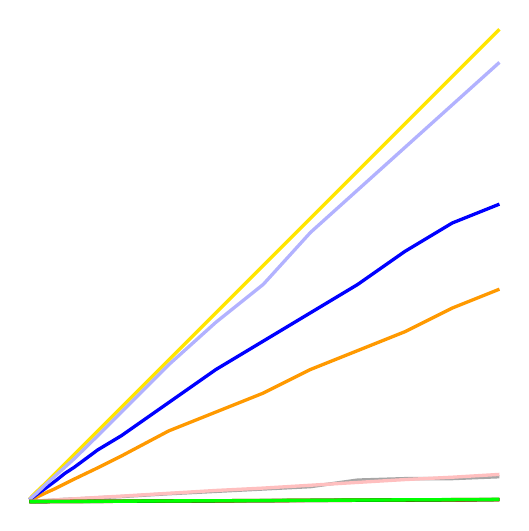
\begin{tikzpicture}[xscale=0.6,yscale=0.6]
		\DrawAxes{steps}{time~(sec)}
		\GridOn
		\TicksOn
		\XAxisText{0.05cm/25}{1cm/}{2cm/1000}{3cm/}{4cm/2000}{5cm/}{6cm/3000}{7cm/}{8cm/4000}
		\XAxisText{9cm/}{10cm/5000}{}{}{}{}{}{}{}
		\YAxisText{0.00cm/0}{1.00cm/280}{2.00cm/560}{3.00cm/840}{4.00cm/1120}{5.00cm/1400}{6.00cm/1680}{7.00cm/1960}{8.00cm/2240}
		\YAxisText{9.00cm/2520}{10.00cm/2800}{}{}{}{}{}{}{}
		% ------- 2D temporal with 512^2 size -------
		\draw[line width=1.2pt,color=red!40!yellow] (0.05cm,0.027cm) -- (0.1cm,0.047cm) -- (0.2cm,0.094cm) -- (0.4cm,0.19cm) -- (0.6cm,0.28cm) -- (0.8cm,0.38cm) -- ( 1cm,0.48cm) -- (1.5cm,0.72cm) -- ( 2cm,0.97cm) -- ( 3cm,1.5cm) -- ( 4cm,1.9cm) -- ( 5cm,2.3cm) -- ( 6cm,2.8cm) -- ( 7cm,3.2cm) -- ( 8cm,3.6cm) -- ( 9cm,4.1cm) -- (10cm,4.5cm);
		\draw[line width=1.2pt,color=red!10!yellow] (0.05cm,0.052cm) -- (0.1cm,0.11cm) -- (0.2cm,0.21cm) -- (0.4cm,0.4cm) -- (0.6cm,0.6cm) -- (0.8cm,0.8cm) -- ( 1cm, 1cm) -- (1.5cm,1.5cm) -- ( 2cm, 2cm) -- ( 3cm, 3cm) -- ( 4cm, 4cm) -- ( 5cm, 5cm) -- ( 6cm, 6cm) -- ( 7cm, 7cm) -- ( 8cm, 8cm) -- ( 9cm, 9cm) -- (10cm,10cm);
		\draw[line width=1.2pt,color=blue] (0.05cm,0.046cm) -- (0.1cm,0.076cm) -- (0.2cm,0.15cm) -- (0.4cm,0.29cm) -- (0.6cm,0.44cm) -- (0.8cm,0.6cm) -- ( 1cm,0.73cm) -- (1.5cm,1.1cm) -- ( 2cm,1.4cm) -- ( 3cm,2.1cm) -- ( 4cm,2.8cm) -- ( 5cm,3.4cm) -- ( 6cm, 4cm) -- ( 7cm,4.6cm) -- ( 8cm,5.3cm) -- ( 9cm,5.9cm) -- (10cm,6.3cm);
		\draw[line width=1.2pt,color=blue!30!white] (0.05cm,0.048cm) -- (0.1cm,0.094cm) -- (0.2cm,0.18cm) -- (0.4cm,0.37cm) -- (0.6cm,0.55cm) -- (0.8cm,0.73cm) -- ( 1cm,0.91cm) -- (1.5cm,1.4cm) -- ( 2cm,1.9cm) -- ( 3cm,2.9cm) -- ( 4cm,3.8cm) -- ( 5cm,4.6cm) -- ( 6cm,5.7cm) -- ( 7cm,6.6cm) -- ( 8cm,7.5cm) -- ( 9cm,8.4cm) -- (10cm,9.3cm);
		\draw[line width=1.2pt,color=gray!70!white] (0.05cm,0.014cm) -- (0.1cm,0.01cm) -- (0.2cm,0.016cm) -- (0.4cm,0.026cm) -- (0.6cm,0.038cm) -- (0.8cm,0.053cm) -- ( 1cm,0.059cm) -- (1.5cm,0.086cm) -- ( 2cm,0.11cm) -- ( 3cm,0.17cm) -- ( 4cm,0.22cm) -- ( 5cm,0.27cm) -- ( 6cm,0.32cm) -- ( 7cm,0.46cm) -- ( 8cm,0.49cm) -- ( 9cm,0.49cm) -- (10cm,0.53cm);
		\draw[line width=1.2pt,color=pink] (0.05cm,0.0099cm) -- (0.1cm,0.011cm) -- (0.2cm,0.017cm) -- (0.4cm,0.028cm) -- (0.6cm,0.04cm) -- (0.8cm,0.051cm) -- ( 1cm,0.063cm) -- (1.5cm,0.092cm) -- ( 2cm,0.12cm) -- ( 3cm,0.18cm) -- ( 4cm,0.24cm) -- ( 5cm,0.29cm) -- ( 6cm,0.35cm) -- ( 7cm,0.41cm) -- ( 8cm,0.47cm) -- ( 9cm,0.52cm) -- (10cm,0.58cm);
		\draw[line width=1.2pt,color=red!70!black] (0.05cm,0.003cm) -- (0.1cm,0.0025cm) -- (0.2cm,0.0029cm) -- (0.4cm,0.0037cm) -- (0.6cm,0.0045cm) -- (0.8cm,0.0053cm) -- ( 1cm,0.0062cm) -- (1.5cm,0.0082cm) -- ( 2cm,0.01cm) -- ( 3cm,0.015cm) -- ( 4cm,0.018cm) -- ( 5cm,0.023cm) -- ( 6cm,0.027cm) -- ( 7cm,0.031cm) -- ( 8cm,0.035cm) -- ( 9cm,0.039cm) -- (10cm,0.043cm);
		\draw[line width=1.2pt,color=red] (0.05cm,0.0068cm) -- (0.1cm,0.0041cm) -- (0.2cm,0.0045cm) -- (0.4cm,0.0054cm) -- (0.6cm,0.0063cm) -- (0.8cm,0.0072cm) -- ( 1cm,0.0083cm) -- (1.5cm,0.011cm) -- ( 2cm,0.013cm) -- ( 3cm,0.017cm) -- ( 4cm,0.022cm) -- ( 5cm,0.027cm) -- ( 6cm,0.031cm) -- ( 7cm,0.036cm) -- ( 8cm,0.04cm) -- ( 9cm,0.045cm) -- (10cm,0.05cm);
		\draw[line width=1.2pt,color=green!50!black] (0.05cm,0.0029cm) -- (0.1cm,0.0026cm) -- (0.2cm,0.0031cm) -- (0.4cm,0.0039cm) -- (0.6cm,0.0048cm) -- (0.8cm,0.0057cm) -- ( 1cm,0.0066cm) -- (1.5cm,0.0088cm) -- ( 2cm,0.011cm) -- ( 3cm,0.016cm) -- ( 4cm,0.02cm) -- ( 5cm,0.024cm) -- ( 6cm,0.029cm) -- ( 7cm,0.033cm) -- ( 8cm,0.038cm) -- ( 9cm,0.042cm) -- (10cm,0.047cm);
		\draw[line width=1.2pt,color=green] (0.05cm,0.0045cm) -- (0.1cm,0.0036cm) -- (0.2cm,0.0041cm) -- (0.4cm,0.0051cm) -- (0.6cm,0.006cm) -- (0.8cm,0.0072cm) -- ( 1cm,0.0079cm) -- (1.5cm,0.01cm) -- ( 2cm,0.013cm) -- ( 3cm,0.018cm) -- ( 4cm,0.022cm) -- ( 5cm,0.027cm) -- ( 6cm,0.032cm) -- ( 7cm,0.036cm) -- ( 8cm,0.041cm) -- ( 9cm,0.046cm) -- (10cm,0.051cm);
	\end{tikzpicture}
	}
}
\begin{tikzpicture}
\DrawLegend
\end{tikzpicture}
\caption{Performance comparison}
\label{fig:Peformance-comparison}
\end{figure}
\nocite{*}
\bibliographystyle{ieeetr} %plain, ieeetr
\bibliography{FDTDMETARef}

\end{paper}
%--------------------------

\end{document}
